\subsubsection{Exercise}

The specification of the controlled system are the following:

\begin{shortitemize}
    \item Phase margin: $\varphi_m = \pi/3$
    \item Crossover frequency: 
        \begin{shortitemize}
            \item Minimum phase system: $\omega_{c,m} = .1$rad/s
            \item Non-minimum phase system: $\omega_{c,nm} = .02$rad/s
        \end{shortitemize}
\end{shortitemize}

As we can see $\omega_{c,nm} \leq .029$ (see Exercise 3.1.2). Therefore the RHP zero will not be a problem.

The controller are designed using the method depicted in the subject. 
We have the following values:

\begin{center}
    \begin{tabular}{|c|cc|}
        \hline
        & $f_1(s)$ & $f_2(s)$ \\
        \hline
        & & \\
        $F_{m}(s)$ &
        $ 1.68 (1 + \frac{1}{5.90s}) $ &
        $ 2.01 (1 + \frac{1}{6.39s}) $  \\ 
        & & \\
        $F_{nm}(s)$ & 
        $ 0.15 (1 + \frac{1}{3.94s}) $ &
        $ 0.14 (1 + \frac{1}{4.81s}) $ \\
        & & \\
       \hline 
    \end{tabular}
\end{center}

Figure \ref{bode321} shows the bode diagrams of the transfer function $L$ for the coupled input--output. The margin and cross-over criteria are fullfilled. Moreover the phase margin for the non-minimum phase system is bigger ($\approx 80^{\circ}$) than the one expected, which is even better.

\begin{figure}[h!b]
    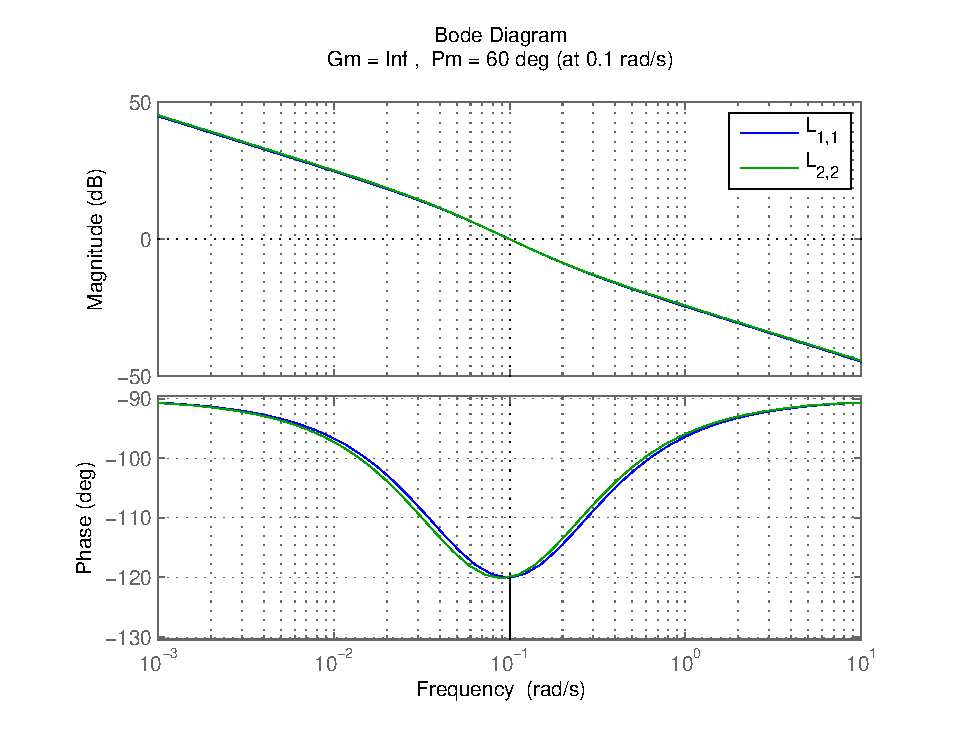
\includegraphics[width=\columnwidth]{fig/Lm321.eps}
    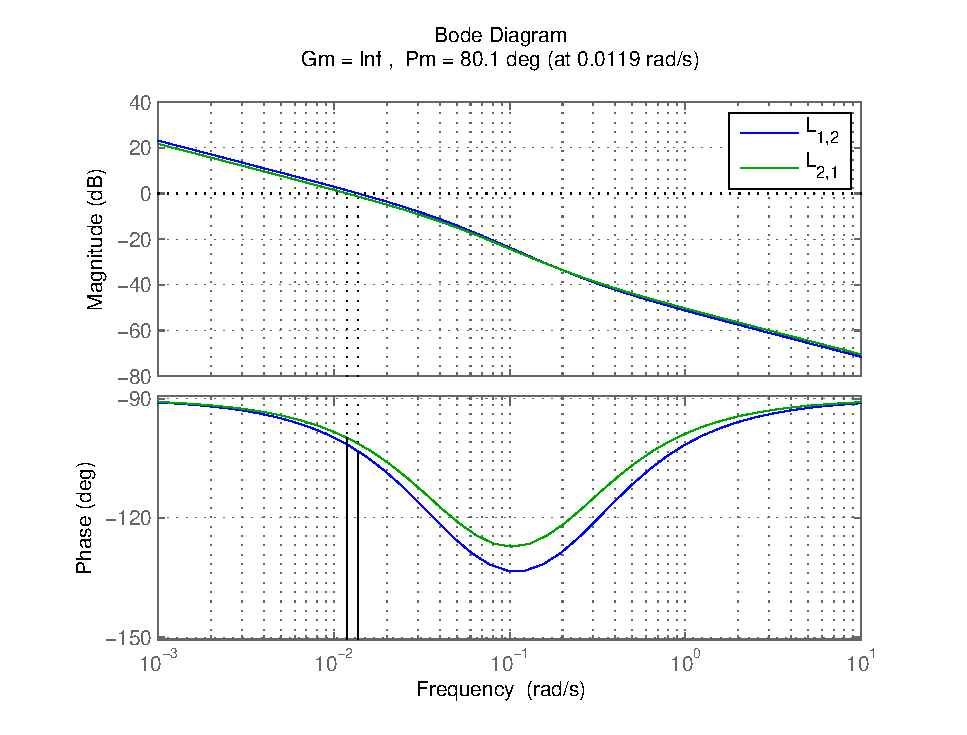
\includegraphics[width=\columnwidth]{fig/Lnm321.eps}
    \caption{Bode diagram of $L$ for the minimum phase system (top) and the non-minimum phase system (bottom)}
    \label{bode321}
    \label{bode321}
\end{figure}
